\chapter{Sviluppo del controllore di temperatura per l'incubatrice neonatale}
\section{Requisiti del controllore di temperatura}
Per poter essere immessa sul mercato, un’incubatrice neonatale deve soddisfare i requisiti previsti da diverse normative
tecniche, tra cui la norma ``IEC 60601-2-19'' \cite{iec_60601_2_19}, sviluppata dalla IEC (International Electrotechnical
Commission), che costituisce il principale riferimento internazionale per questa tipologia di dispositivi. La norma è stata
successivamente recepita in ambito europeo dal CEN (Comitato europeo di normazione) e dal CENELEC (Comitato europeo di
normazione elettrotecnica), dando origine alla norma ``EN IEC 60601-2-19''.

Per la progettazione del controllore è stata assunta come riferimento la versione britannica della norma,
``BS EN IEC 60601-2-19:2021+A1:2023'' \cite{bs_60601_2_19}. Tale documento è tecnicamente identico alla norma
``IEC 60601-2-19:2020'' con l'integrazione dell'emendamento A1:2023.

Analizzando le parti relative al controllo della temperatura delle incubatrici neonatali, si possono individuare i seguenti
requisiti principali:

\begin{itemize}
	\item sensore posizionato al centro della culla, a 10 cm dalla base del materasso
	\item funzionalità del controllore con temperature esterne comprese tra i 20°C e i 30°C
	\item setpoint compreso tra 35 e 37°C, almeno 3°C sopra la temperatura ambiente
	\item il setpoint impostabile dall'operatore non deve superare i 37°C, è permesso impostare una temperatura fino
	a 39°C, ma la norma impone che questo avvenga esclusivamente tramite un'azione intenzionale e separata da parte
	dell'operatore
	\item warm-up time: tempo impiegato per arrivare a +11°C dalla temperatura ambiente, ad esempio 25°C -> 36°C, deve
	rientrare entro il 20\% del valore dichiarato nelle istruzioni
	\item una volta raggiunta la temperatura target (Steady Temperature Condition - STC), questa non deve variare per
	più di 1°C nell'arco di un'ora, micro fluttuazioni di 0.5°C sono ammesse
	\item overshoot transitorio non deve superare i 2°C
	\item riacquisizione della condizione di regime (steady state) entro 15 minuti da un eventuale disturbo
\end{itemize}

\section{Controllore ad isteresi}
\subsection{Principio di funzionamento di un controllore ad isteresi}
\subsection{Implementazione del controllore ad isteresi nel firmware}
\subsection{Test di funzionamento con grafico e prestazioni}

\begin{figure}[htbp]
	\centering
	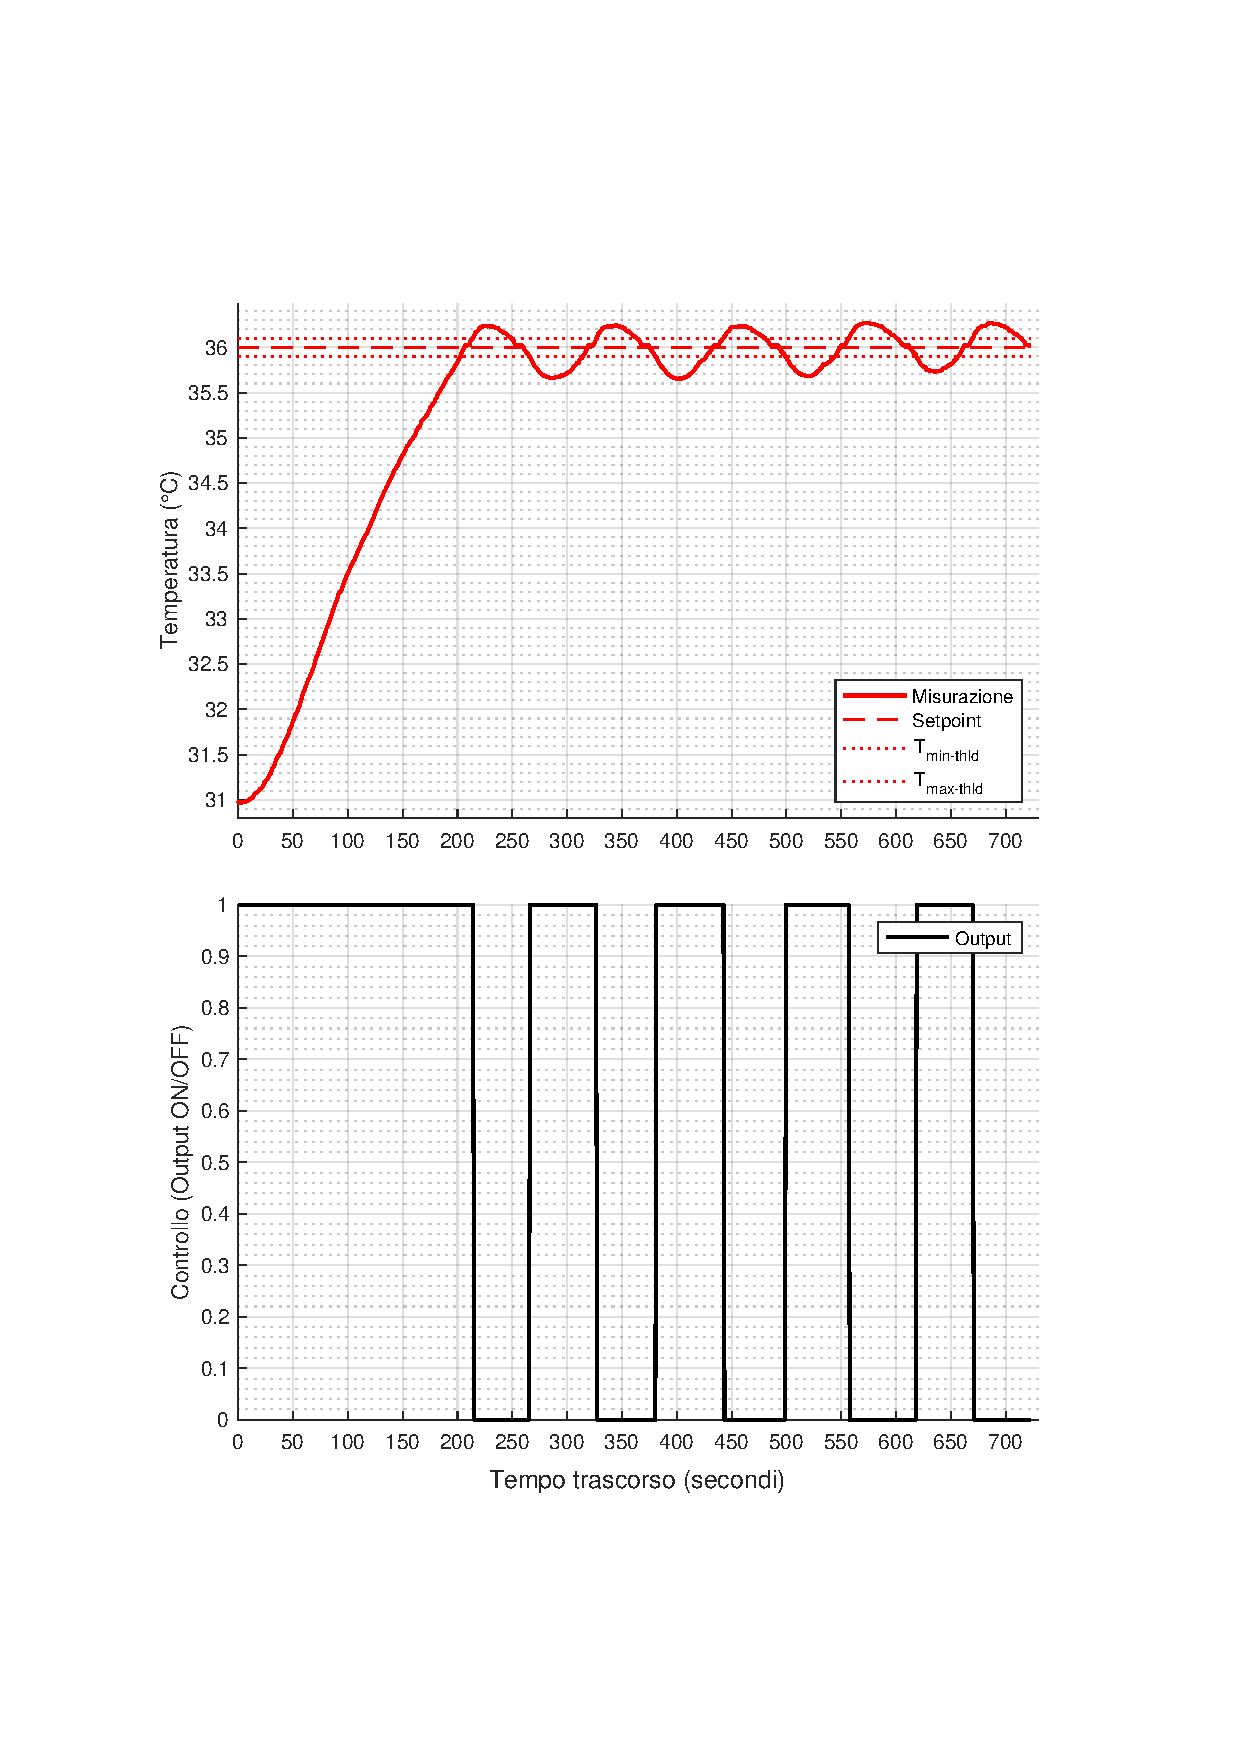
\includegraphics[width=0.9\textwidth, trim={2.5cm 4cm 2.5cm 4cm}, clip]{immagini/3_isteresi.pdf}
	\caption[Grafico del setpoint del controllore ad isteresi]{Grafico del raggiungimento e mantenimento del setpoint
	di temperatura ottenuto con il controllore ad isteresi.}
	\label{fig:isteresi}
\end{figure}

\newpage

\section{Controllore PID}
\subsection{Principio di funzionamento di un controllore PID}
\subsection{Implementazione del controllore PID nel firmware}
\subsubsection{Salvataggio degli errori e delle misurazioni nel buffer}
\subsubsection{Aggiornamento dello stato}
\subsubsection{Gestione del ciclo pwm}
\subsubsection{Sistema di anti-windup}
\subsubsection{Derivative on measurement}
\subsection{Test di funzionamento con grafico e prestazioni}


parametri ottimali individuati:
\begin{itemize}
	\item kp = 55, ki = 0.40, kd = 1000
	\item kp = 55, ki = 0.35, kd = 1200
	\item kp = 60, ki = 0.4, kd = 1500
\end{itemize}

prestazioni richieste:
\begin{itemize}
	\item rise time
	\item settling time
	\item overshoot
\end{itemize}

\begin{figure}[htbp]
	\centering
	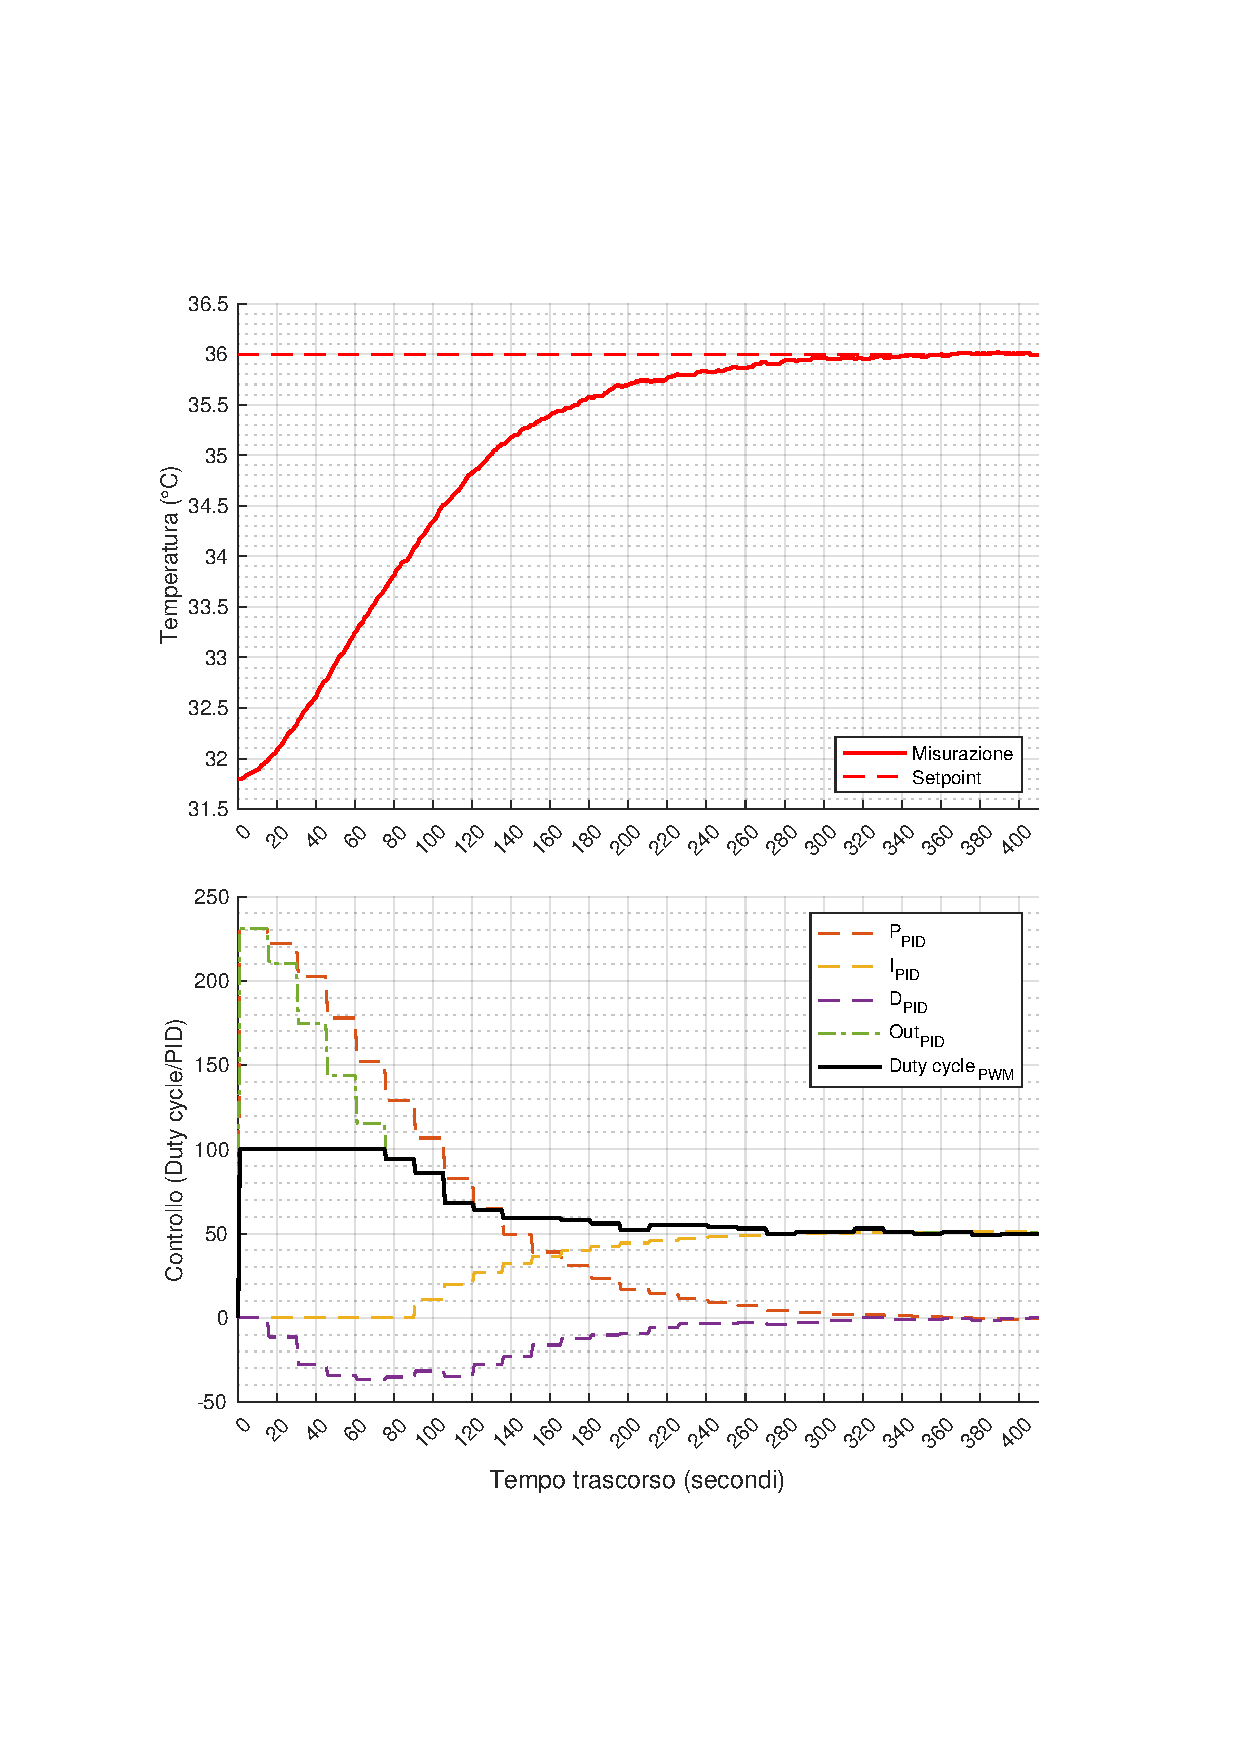
\includegraphics[width=0.9\textwidth, trim={2.5cm 4cm 2.5cm 4cm}, clip]{immagini/3_pid_1_1.pdf}
	\caption[Grafico del setpoint del controllore PID]{Grafico del raggiungimento e mantenimento del setpoint di temperatura
	ottenuto con il controllore PID con parametri Kp=55, Ki=0.35, Kd=1200.}
	\label{fig:pid_gradino}
\end{figure}

\begin{figure}[htbp]
	\centering
	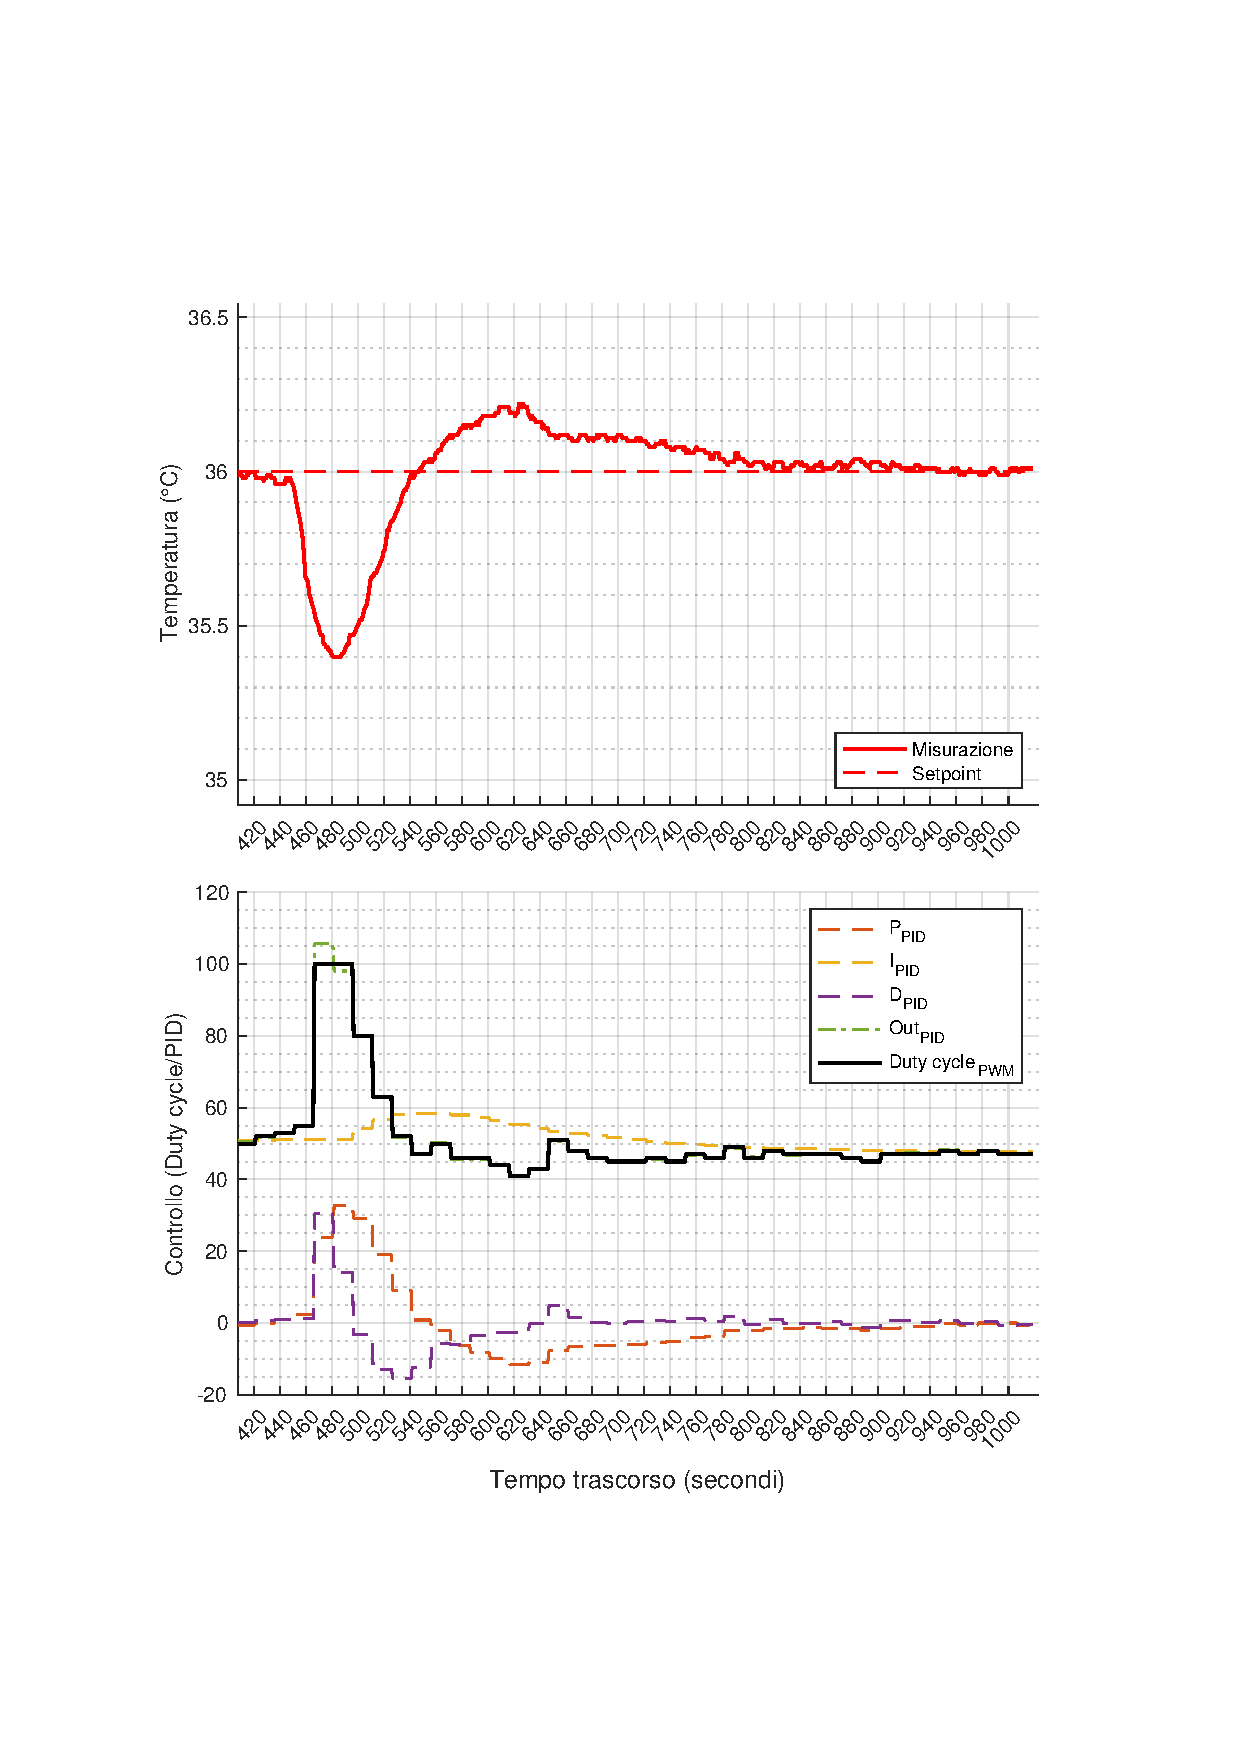
\includegraphics[width=0.9\textwidth, trim={2.5cm 4cm 2.5cm 4cm}, clip]{immagini/3_pid_1_2.pdf}
	\caption[Grafico della perturbazione del controllore PID]{Grafico del ripristino del setpoint di temperatura dopo un
	disturbo esterno, ottenuto con il controllore PID con parametri Kp=55, Ki=0.35, Kd=1200.}
	\label{fig:pid_perturbazione}
\end{figure}

\section{Confronto tra controllore ad isteresi e PID}
